\documentclass[11pt, conference]{IEEEtran}
\usepackage[spanish]{babel}
\usepackage[utf8]{inputenc}
\usepackage{amsmath}
\usepackage{amsfonts}
\usepackage{cite}
\usepackage{amssymb}
\usepackage{graphicx}
\renewcommand{\labelenumii}{\theenumii}
\renewcommand{\theenumii}{\theenumi.\arabic{enumii}.}
\addtocounter{tocdepth}{-1}

\begin{document}
	\title{\bf Kevin Jhomar Sanchez Sanchez}
	\maketitle
	
\section{Logaritmos}
\[\log_ba = c\longrightarrow b^c=a\]
\[\log_b1 = 0\]
\[\log_bb = 1\]
\[\log_bb^n = n,\ con\ b\neq 1\]
\[\log_b(a*c) = \log_ba + \log_bc\]
\[\log_b\left(\frac{p}{q}\right) = \log_bp + \log_bq\]
\[\log_ac^n = n\log_ac\]
\[\log_b\sqrt[n]{a^m} = \frac{m}{n}\cdot\log_ba\]
\[\log_pa = \frac{\log_ba}{\log_bp}\]
\section{Logaritmos Neperianos}
\[\ln1=0\]
\[\ln e=1\]
\[\ln e^n=n\]
\[\ln(x\cdot y)=\ln(x) + \ln(y)\]
\[\ln\left(\frac{x}{y}\right)=\ln(x) - \ln(y)\]
\[\ln x^n=n\ln(x)\]
\[\ln\sqrt[n]{x}=\frac{1}{n}\ln x\]
\section{Funcion Exponencial}
\[\ln e^x=x\]
\[e^{\ln x}=x\]
\[e^0=1\]
\[e^{u+v}=e^u\cdot e^v\]
\[e^{u-v}=\frac{u}{v}\]
\[e^{-v}=\frac{1}{e^v}\]
\section{Identidades Trigonometricas}
\[sen^2x+cos^2x = 1\]
\[tan^2x+1 = sec^2x\]
\[cot^2x+1 = csc^2x\]
\[senx+cscx = 1\]
\[cosx+secx = 1\]
\[tanx+cotx = 1\]
\[tanx = \frac{senx}{cosx}\]
\[cotx = \frac{cosx}{senx}\]
\[secx = \frac{1}{cosx}\]
\[cscx = \frac{1}{senx}\]
\[sen(x\pm y) = senx\cdot cosy \pm cosx\cdot seny\]
\[cos(x\pm y) = cosx\cdot cosy \mp senx\cdot seny\]
\[tan(x\pm y) = \frac{tanx\pm tany}{1\mp tanx\cdot tany}\]
\[sen2x=2senx\cdot cosx\]
\[cos2x=cos^2x-sen^2x\]
\[cos2x=2cos^2x-1\]
\[cos2x=1-2sen^2x\]
\pagebreak
\onecolumn
\section{Triangulos Notables}	
\begin{figure}[h]
	\begin{center}
		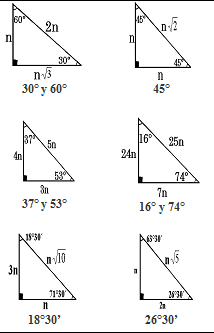
\includegraphics[scale=1]{2.png}
	\end{center}
\end{figure}

\section{Tabla de Angulos}
\begin{figure}[h]
	\begin{center}
		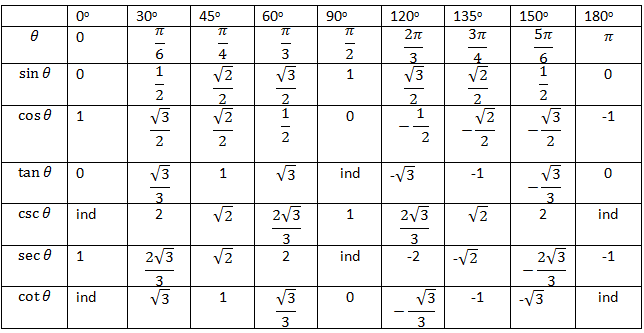
\includegraphics[scale=0.64]{1.png}
	\end{center}
\end{figure}	
	

\end{document}